%%%%%%%%%%%%%%%%%%%%%%%%%%%%%%%%%%%%%%%%%%%%%%%%%%%%%%%%%%%%%%%%%%%%%%%%%%%%
% AGUJournalTemplate.tex: this template file is for articles formatted with LaTeX
%
% This file includes commands and instructions
% given in the order necessary to produce a final output that will
% satisfy AGU requirements, including customized APA reference formatting.
%
% You may copy this file and give it your
% article name, and enter your text.
%
% guidelines and troubleshooting are here: 

%% To submit your paper:
\documentclass{agujournal2019}
\usepackage{url} %this package should fix any errors with URLs in refs.
\usepackage{lineno}
\usepackage[inline]{trackchanges} %for better track changes. finalnew option will compile document with changes incorporated.
\usepackage{soul}
\linenumbers
\usepackage{microtype}
\usepackage{lmodern}
\usepackage{changepage}
%%%%%%%
% As of 2018 we recommend use of the TrackChanges package to mark revisions.
% The trackchanges package adds five new LaTeX commands:
%
%  \note[editor]{The note}
%  \annote[editor]{Text to annotate}{The note}
%  \add[editor]{Text to add}
%  \remove[editor]{Text to remove}
%  \change[editor]{Text to remove}{Text to add}
%
% complete documentation is here: http://trackchanges.sourceforge.net/
%%%%%%%

\draftfalse

%% Enter journal name below.
%% Choose from this list of Journals:
%
% JGR: Atmospheres
% JGR: Biogeosciences
% JGR: Earth Surface
% JGR: Oceans
% JGR: Planets
% JGR: Solid Earth
% JGR: Space Physics
% Global Biogeochemical Cycles
% Geophysical Research Letters
% Paleoceanography and Paleoclimatology
% Radio Science
% Reviews of Geophysics
% Tectonics
% Space Weather
% Water Resources Research
% Geochemistry, Geophysics, Geosystems
% Journal of Advances in Modeling Earth Systems (JAMES)
% Earth's Future
% Earth and Space Science
% Geohealth
%
% ie, \journalname{Water Resources Research}

\journalname{Earth's Future}


\begin{document}

%%%%%%%%%%%%%%%%%%%%%%%%%%%%%%%%%%%%%%%%%%%%%%%
%  TITLE
%
% (A title should be specific, informative, and brief. Use
% abbreviations only if they are defined in the abstract. Titles that
% start with general keywords then specific terms are optimized in
% searches)
%
%%%%%%%%%%%%%%%%%%%%%%%%%%%%%%%%%%%%%%%%%%%%%%%

% Example: \title{This is a test title}

\title{Intensifying renewable energy droughts in the Western U.S. amid evolving infrastructure and climate}

%%%%%%%%%%%%%%%%%%%%%%%%%%%%%%%%%%%%%%%%%%%%%%%
%
%  AUTHORS AND AFFILIATIONS
%
%%%%%%%%%%%%%%%%%%%%%%%%%%%%%%%%%%%%%%%%%%%%%%%

% Authors are individuals who have significantly contributed to the
% research and preparation of the article. Group authors are allowed, if
% each author in the group is separately identified in an appendix.)

% List authors by first name or initial followed by last name and
% separated by commas. Use \affil{} to number affiliations, and
% \thanks{} for author notes.
% Additional author notes should be indicated with \thanks{} (for
% example, for current addresses).

% Example: \authors{A. B. Author\affil{1}\thanks{Current address, Antartica}, B. C. Author\affil{2,3}, and D. E.
% Author\affil{3,4}\thanks{Also funded by Monsanto.}}

\authors{C. Bracken\affil{1}, N. Voisin\affil{1}\affil{2}, K. Mongird\affil{1}, C. D. Burleyson\affil{1}, K. Oikonomou\affil{1}}


% \affiliation{1}{First Affiliation}
% \affiliation{2}{Second Affiliation}
% \affiliation{3}{Third Affiliation}
% \affiliation{4}{Fourth Affiliation}

\affiliation{1}{Pacific Northwest National Laboratory, Richland, WA USA}
\affiliation{2}{University of Washington, Seattle, WA USA}
%(repeat as many times as is necessary)


% Corresponding author mailing address and e-mail address:

% (include name and email addresses of the corresponding author.  More
% than one corresponding author is allowed in this LaTeX file and for
% publication; but only one corresponding author is allowed in our
% editorial system.)

% Example: \correspondingauthor{First and Last Name}{email@address.edu}

\correspondingauthor{Cameron Bracken}{cameron.bracken@pnnl.gov}



%%%%%%%%%%%%%%%%%%%%%%%%%%%%%%%%%%%%%%%%%%%%%%%
% KEY POINTS
%%%%%%%%%%%%%%%%%%%%%%%%%%%%%%%%%%%%%%%%%%%%%%%
%  List up to three key points (at least one is required)
%  Key Points summarize the main points and conclusions of the article
%  Each must be 140 characters or fewer with no special characters or punctuation and must be complete sentences

% Example:
% \begin{keypoints}
% \item	List up to three key points (at least one is required)
% \item	Key Points summarize the main points and conclusions of the article
% \item	Each must be 140 characters or fewer with no special characters or punctuation and must be complete sentences
% \end{keypoints}

\begin{keypoints}
\item The severity of compound wind and solar energy droughts will increase as more wind and solar resources are built. 
\item Climate increases the variability of future compound wind and solar energy drought severity. 
%\item The average duration of compound energy droughts is not expected to change in the future. 
\item Compound wind and solar energy droughts are expected to affect fewer load balancing regions simultaneously in the future.
\end{keypoints}

%%%%%%%%%%%%%%%%%%%%%%%%%%%%%%%%%%%%%%%%%%%%%%%
%
%  ABSTRACT and PLAIN LANGUAGE SUMMARY
%
% A good Abstract will begin with a short description of the problem
% being addressed, briefly describe the new data or analyses, then
% briefly states the main conclusion(s) and how they are supported and
% uncertainties.

% The Plain Language Summary should be written for a broad audience,
% including journalists and the science-interested public, that will not have 
% a background in your field.
%
% A Plain Language Summary is required in GRL, JGR: Planets, JGR: Biogeosciences,
% JGR: Oceans, G-Cubed, Reviews of Geophysics, and JAMES.
% see http://sharingscience.agu.org/creating-plain-language-summary/)
%
%%%%%%%%%%%%%%%%%%%%%%%%%%%%%%%%%%%%%%%%%%%%%%%

%% \begin{abstract} starts the second page

\begin{abstract}
If renewable energy resources continue to become a larger part of the generation mix in the United States (U.S.), so does the potential impact of prolonged periods of low wind and solar generation, known as variable renewable energy (VRE) droughts. In such a future, naturally occurring VRE droughts need to be evaluated for their potential impact on grid reliability. This study is the first of its kind to examine the impacts of compound VRE energy droughts in the Western U.S. across a range of potential future climate and infrastructure scenarios. We find that compound VRE drought severity will increase significantly in the future, primarily due to the dramatic increase in wind and solar generation needed in some future infrastructure scenarios. We find that in our potential future climate scenario, the variability of energy drought severity increases, which has implications for sizing energy storage necessary for mitigating drought events. We also examine the spatial patterns of compound VRE drought events that effect multiple regions of the grid simultaneously. These co-occurring events have distinct spatial patterns depending on the season. We observed overall fewer connected events in the future with the combined effect of climate and infrastructure changes, although in the fall we observe a climate-induced shift toward events which impact more regions simultaneously. 
\end{abstract}

%\section*{Plain Language Summary}
%Enter your Plain Language Summary here or delete this section.

%Here are instructions on writing a Plain Language Summary: 

%https://www.agu.org/Share-and-Advocate/Share/Community/Plain-language-summary


%%%%%%%%%%%%%%%%%%%%%%%%%%%%%%%%%%%%%%%%%%%%%%%
%
%  BODY TEXT
%
%%%%%%%%%%%%%%%%%%%%%%%%%%%%%%%%%%%%%%%%%%%%%%%

%%% Suggested section heads:
% \section{Introduction}
%
% The main text should start with an introduction. Except for short
% manuscripts (such as comments and replies), the text should be divided
% into sections, each with its own heading.

% Headings should be sentence fragments and do not begin with a
% lowercase letter or number. Examples of good headings are:

% \section{Materials and Methods}
% Here is text on Materials and Methods.
%
% \subsection{A descriptive heading about methods}
% More about Methods.
%
% \section{Data} (Or section title might be a descriptive heading about data)
%
% \section{Results} (Or section title might be a descriptive heading about the
% results)
%
% \section{Conclusions}


\section{Introduction}


% main points:
% - VRE droughts pose a risk to the future grid
% - There are lots of historical studies but very few future studies (only one actually)
%- change this first sentence with drastic increase in the recen tpast and in some scenario projection, it may keep increasing ( same references)
Renewable generation capacity in the U.S. has dramatically increased in the recent past \cite{Browning_2023,Ou2023,Ou2024}. As variable renewable resources become a larger part of the generation mix in the U.S., so does the potential impact of prolonged periods of low wind and solar generation, known as variable renewable energy (VRE) droughts \cite{Bracken2024}. VRE droughts may last for hours to months depending on the data used to define the droughts. The drought is said to occur when the generation falls below some predefined threshold. A compound drought occurs when 2 or more renewable generating sources are in drought conditions simultaneously. In the contemporary grid, VRE droughts can be mitigated by increased generation from other, often carbon intensive sources \cite{van_der_Wiel_2019a,Raynaud2018,Rife2016}. A high renewable grid cannot rely on fossil-fuel based generation, so VRE droughts must be mitigated with local energy storage or by inter-regional transfers of energy \cite{Dyreson2022,Doering2023}. In this high renewable future, VRE droughts need to be considered when planning for storage and transmission of the future grid so as not to pose a threat to grid reliability. 

%A growing body of literature has examined energy droughts in a number of contexts and geographic locations. However, as \citeA{Kittel2024} point out in their review paper, the terminology and methodologies employed to analyze energy droughts are somewhat inconsistent. They propose the term variable renewable energy (VRE) drought to refer to low periods of energy production, which for the purposes of this paper we will shorten to energy drought, the intended meaning is the same. 

Historical VRE droughts have been the focus of numerous studies which showed that they are highly spatially variable and require detailed regional studies to understand their properties. Wind energy droughts, \cite{Cannon_2015, Potisomporn_2021, Potisomporn_2023, Potisomporn_2024, Abdelaziz_2024, Leahy_2012, Patlakas_2017, Ohlendorf_2020, Kay_2023}, compound VRE energy droughts, which involve two or more resource types (wind, solar, and sometimes hydropower) \cite{Gburcik2013,Otero2022,Bloomfield2020b,Bett2016,Otero2022a,Raynaud2018,Miglietta2017,Bloomfield2020c,Francois2016c,van_der_Wiel_2019a,GonzalezSalazar2022,FerrazdeAndradeSantos2020a,Bloomfield2022,Brown2021,Doering2018,Rinaldi2021,Amonkar2022,Bracken2024,Zheng_2024}, meteorological drivers for energy droughts \cite{Tong2021,Engeland2017a,Mohammadi2018,Lledo2018,van_der_Wiel_2019a,van_der_Wiel_2019b}, and the reliability of complementary renewable systems (e.g., complementary hydro and wind systems) \cite{Jurasz2018,Solomon2016,Potrc2022} have been the focus of many studies. Despite this growing body of literature, research to date has been either purely atmospheric and lacking a translation to the power sector, or has been based on current or historical infrastructure, climate, and load and lacking insight into future grid and climate conditions. 

The gap in energy supply left when renewables cannot fully meet demand, known as positive residual load (PRL) events \cite{Kittel2024}, has the potential for significant grid impacts and requires detailed knowledge of a particular system to quantify. Historical PRL events have been studied in Europe \cite{Raynaud2018, Otero2022, Otero2022a, Fran_ois_2022,Ruhnau_2022, van_der_Wiel_2019a, van_der_Wiel_2019b} and North America \cite{Rinaldi2021, Bracken2024}, but future conditions have not yet been evaluated at such high spatio-temporal resolution because they require future infrastructure, climate and load projections. 

While future projections of wind and solar energy supply have been studied \cite{Jung_2022,Dutta_2022,Gernaat_2021}, the literature on future impacts on VRE droughts is limited. \citeA{Kapica_2024} evaluate changes in the frequency of wind and solar energy droughts across Europe with 8 Coupled Model Intercomparison Project (CMIP) 5 models and 2 Representative Concentration Pathway (RCP) scenarios. They find a high degree of variability in the change signal spatially and across the climate models. However, the study only examines changes in the frequency, missing intensity and duration of energy droughts, and does not incorporate future grid characteristics such as the total capacity of renewable generation in the system. 

Finally, while climate resilient power grid infrastructure planning focuses on extreme events (FERC order 896), energy droughts have the potential to disrupt markets across regions \cite{Hill_2021} and may require incentives to manage local multi-day storage in the future \cite{Bracken2024}. To support this planning for climate-resilient grid operations, there is a need to characterize how those energy droughts will evolve in the future. To this end, in this study we seek to understand how compound VRE droughts will change under evolving power grid infrastructure and climate conditions in the Western U.S. Specifically, we develop hourly wind and solar data for evolving infrastructure and characterize VRE droughts at the balancing authority (BA) scale which is the scale where, in the U.S., net load (total load minus wind and solar) needs to be locally balanced at all times. This study is organized as follows: Section 2 describes our data and methods. Section 3 presents evolving characteristics of energy droughts. In Section 4 we discuss the limitations and specifically the implications for power grid reliability studies and how the insights can be used for storage and transmission planning studies. 

\section{Data and Methods}

Examining future VRE droughts requires a combination of future climate conditions and future power grid infrastructure projections. A framework is needed to estimate future energy needs, site new infrastructure, retire old or non-compliant infrastructure, and simulate future generation. This framework involves several models run in an iterative process (Figure \ref{fig:flowchart}). Initially, an integrated assessment model is run at a 5-year time step from (2025-2050) to determine future loads and the generation capacity \cite{Ou2024}. Unlike most capacity expansion models which operate on a zonal-scale, this model generates state-level capacity expansion plans based on our future socioeconomic scenario. The state-level capacity expansion plans are then downscaled into individual renewable plant siting locations using a geospatial power plant siting model \cite{Vernon_2021}. Sitings in each timestep represent new power plants that are developed across the 5-year range and operational by the timestep. An iterative process is then conducted for each 5-year timestep where a production cost model (PCM) of the Western U.S. grid is run to determine energy prices using new and existing infrastructure in each location. Energy prices from the PCM are then passed to the power plant siting model to inform optimal siting locations in the next timestep. Areas with higher energy prices, which can occur due to transmission congestion and grid stress, incentivize new siting in these locations moving forward. The iteration between the PCM and the siting model is repeated at every 5-year timestep until 2050. This study focuses on the the newly sited wind and solar generation and its vulnerability to energy droughts. %More details on the infrastructure design can be found in \cite{Mongird2024}. 

\begin{figure}
\noindent
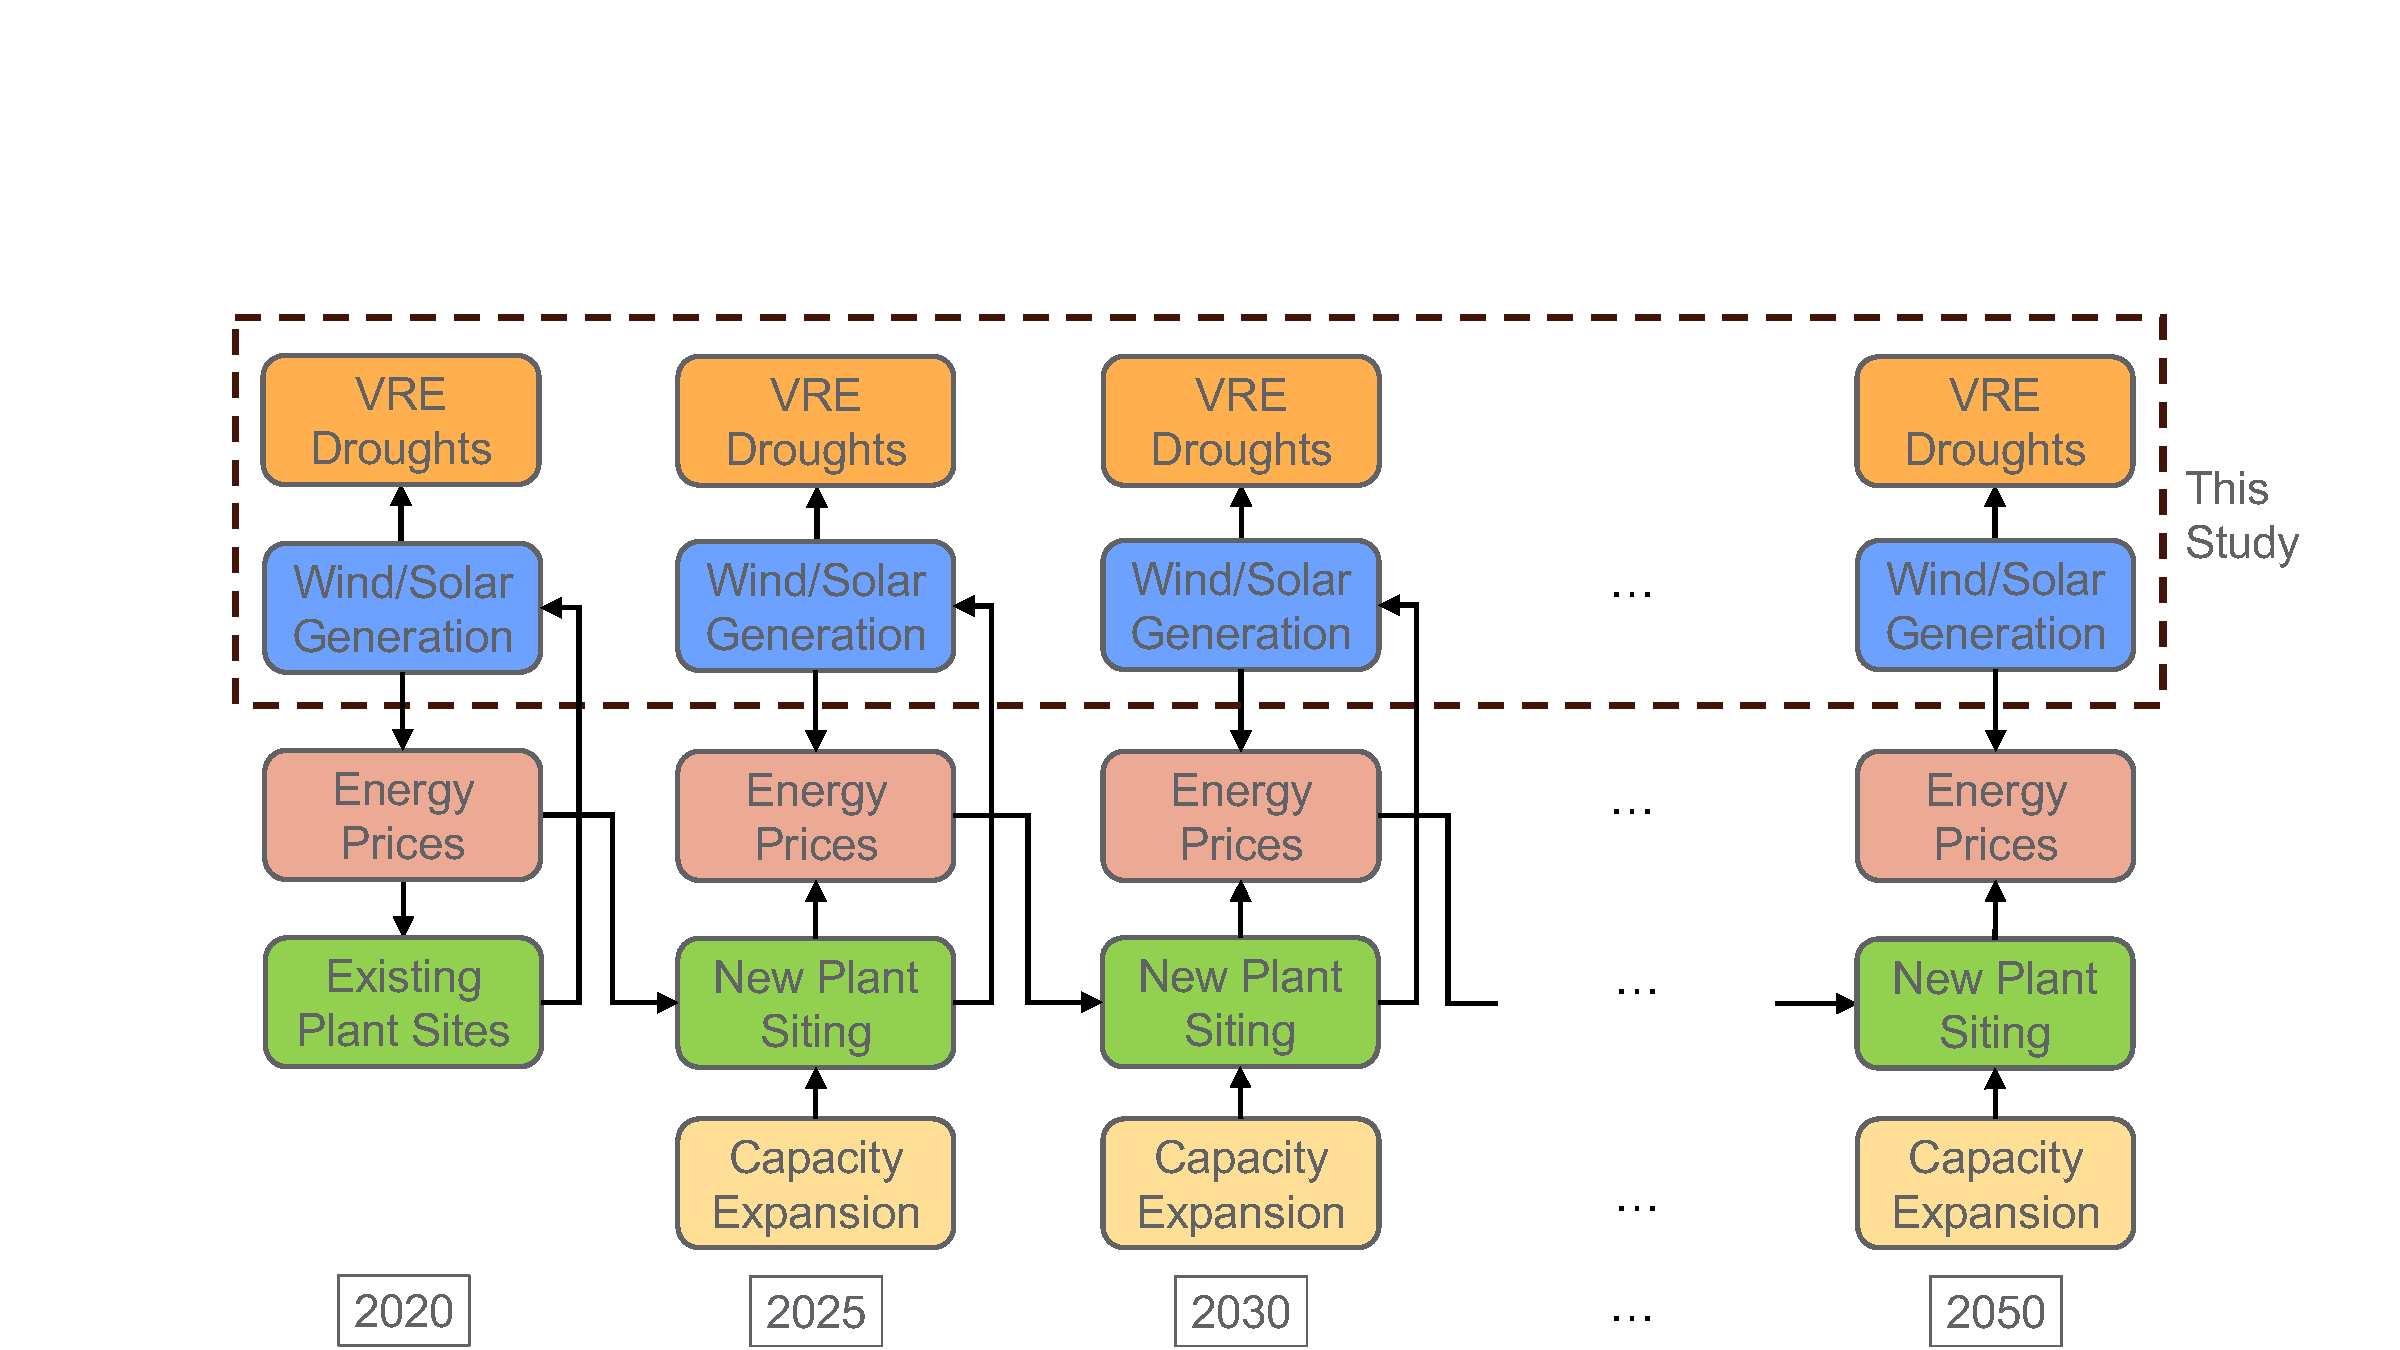
\includegraphics[width=\textwidth]{1-flowchart2}
\caption{Iterative model chain to site new wind and solar infrastructure out to 2050.}
\label{fig:flowchart}
\end{figure}

\subsection{Meteorology Data}
To drive the meteorological variability in this study we leverage a set of Thermodynamic Global Warming (TGW) simulations for the U.S. \cite{Jones2022,Jones2023}. These simulations start with 40 years of historical (1980-2019) weather and then "replays" the hour-to-hour variability of weather across all 40 years with additional warming applied to the boundary conditions of the dynamic downscaling model to reflect the average warming level from a range of climate models. Average warming levels were derived for two emissions pathways (RCPs 4.5 and 8.5) and for climate models that were colder and warmer than the multi-model mean. The future expansion plans and loads used in this study are based on the rcp85hotter scenario in the TGW data (i.e., the hottest scenario). While RCP8.5 is the highest emission scenario represented in the global climate models, it is nonetheless a likely scenario over near- to midterm time horizons having good agreement with historical observations and future emissions under current policy \cite{Schwalm2020}. In addition, the reduction in the effects of cooling aerosols due to lower cabon concentrations in the atmosphere \cite{Dreyfus2022, Smil2013} and positive feedback loops \cite{Ripple2023,Moller2024}. We note that the GODEEEP project and this study only assume lower carbon emissions for the U.S. and not globally. 

\subsection{Future infrastructures}
The future power grid buildouts are developed using the GCAM-USA model, a version of the Global Change Analysis Model (GCAM) with a state-level representation of the US. GCAM-USA simulates interacting markets for energy, water, and land in response to specific scenario drivers. This multisectoral model is used to evaluate market, policies, socio-economic change and technology innovations. A multisectoral load projection as well as a capacity expansion model are parts of the energy sector representations. Two future buildout scenarios are evaluated in this study. The business-as-usual scenario represents the technology, incentives and state goals as of 2020. The high renewable scenario follows this business-as-usual guidance and further drives the model by imposing requirements for a high renewable power grid by 2035 and a high renewable economy by 2050 across the US. The GCAM-USA runs in this experiment used the Shared Socioeconomic Pathways (SSP) 2 scenario for socioeconomic and population forcing and the rcp85hotter TGW climate scenario. 

GCAM-USA simulates the annual total demand for electricity at the state-level \cite{Khan_2021,Binsted2022}. The high renewable economy by 2050 policy in particular drives significant electrification in multiple sectors and a dramatic increase in electricity demand \cite{Ou2023}. Other outcomes include state-scale generation portfolios at a 5-year time step \cite{Ou2023}. Only the high renewable scenario is presented in the main manuscript while the business as usual is presented in supplemental material. GCAM-USA projections of a high renewable economy by 2050 is on par with other projections by other models \cite{Browning_2023}.  

State-level annual total loads from GCAM-USA were shaped into hourly demand time-series for each BA using the Total ELectricity Loads (TELL) model \cite{McGrath2022}. TELL estimates of the hourly demand for electricity using the hour-to-hour variations in population-weighted meteorology in each BA in the TGW data \cite{Burleyson2023}. Details of the TELL modeling approach are provided in \cite{Burleyson2024}. While not used in the drought analytics, this step is needed to develop the price simulations needed to inform high resolution siting.  

\subsection{Infrastructure and Renewable Siting}
New solar and wind facility locations in each infrastructure expansion (GCAM-USA) time step were determined using the Capacity Expansion Regional Feasibility (CERF) geospatial and economic power plant siting model \cite{Vernon_2021}. CERF downscales regional capacity expansion plans from zonal models, here GCAM-USA, to determine 1 km resolution power plant locations by integrating high-resolution geospatial siting suitability data with an economic algorithm \cite{Vernon_2023,Mongird_2024}. The 1 km solar photovoltaic, concentrating solar power, onshore wind, and offshore wind sitings from CERF were combined with an gridded hourly climate dataset and processed by the renewable generation model reV to determine hourly solar and wind generation at individual sited power plants and then aggregated to the BA scale. Those sitings are not processed through licensing and other local adoption processes, rather they indicate where plants could placed be in order to inform energy drought and equity studies. 

\subsection{Renewable Generation Modeling}

Hourly renewable generation is produced for existing and future sited plants using the reV model \cite{Maclaurin2019, Buster2023}. reV is a collection of tools for modeling renewable systems, of which generation is one component. The specific generation models used are windpower \cite{windpower} for wind and PVWatts \cite{pvwatts5} for solar. The variables needed for the wind power model are pressure, temperature, wind speed, and wind direction and the variables needed for the solar model are pressure, temperature, wind speed, and solar radiation. Some prepossessing is necessary to prepare the renewable model inputs from raw meteorology data. For example, the upper level atmospheric data needs to be interpolated to the proper hub height for each wind turbine and solar radiation needs to be broken into its three components: global horizontal, diffuse normal, and direct normal irradiance. Full details of the meteorological data prepossessing are described in \citeA{Bracken2024} along with a historical evaluation in \citeA{Campbell2024}. 

\subsection{Energy Prices}
Energy prices for each iteration of infrastructure is calculated using the commercial production cost modeling (PCM) tool, GridView \cite{hitachi_gridview}. 
GridView is a chronological unit commitment (UC) and economic dispatch (ED) model that minimizes power systems’ operating costs of meeting electricity demand and reserve requirements while simultaneously satisfying a wide variety of operating constraints. These constraints consist of unit-specific constraints (e.g., maximum/maximum capacity limits, minimum up and down times, ramping limits) and system-wide constraints (e.g., transmission line capacity limits, interface capacity limits, operating reserves, emission constraints, hurdle rates). Operating costs largely consist of fuel costs, variable operating and maintenance costs, and start-up/shut-down costs. To model the Western Interconnection grid, GridView leverages the Western Electricity Coordinating Council (WECC) 2030 Anchor Data Set (ADS) case \cite{wecc2021a}, which is backcasted to the starting iteration of infrastructure, 2020. For each subsequent infrastructure iteration in 5 year increments, the GridView database is updated with the downscaled regional capacity expansion decisions, hourly load, and hourly renewable energy profiles.

\subsection{Experimental Setup}

For each iteration of infrastructure (2020, 2025, 2030, 2035, 2040, 2045, and 2050), renewable hourly wind and solar generation data is produced using both 40 years of historical weather (1980-2019) and 40 years of future weather (2020-2059). Due to the way the TGW data is constructed, each historical year is paired with a chronologically equivalent year that occurs 40 years in the future (for example, 2059 is the future equivalent of 2019 with an added warming signal applied). Compound VRE droughts are identified independently for each 40 year period, both historical and future (see the next section for details). For each infrastructure year, the historical period provides a baseline set of VRE droughts and isolates just the infrastructure impact since no climate signal is imposed on the historical period. The future period provides a set of droughts that include both the effects of evolving infrastructure and future climate. By taking the difference between the historical and future periods, we can isolate the climate impact on energy droughts for each infrastructure year. This setup is identical for both the business-as-usual and high renewable scenario. 

%In practice, many of the plants are similar across infrastructure years so each set of wind and solar plants do not need to be re-run for each infrastructure year. Sets of plants are combined into infrastructure year groups via post-processing. 

\subsection{Identification of Compound VRE Droughts}

VRE droughts are expected at the plant scale due to natural variability in the weather and climate. Here we examine the aggregate behavior of VRE droughts at the BA scale where wind and solar resources are considered as non-dispatchable due to their intermittency and net load (load minus wind and solar) needs to be balanced at all times first within that region and eventually with imports. This scale is thus critical for informing storage and transmission planning studies. While there are 47 BAs in the Western U.S. interconnect, the study focus on the 18 BAs which contain both wind and solar generation (Figure \ref{fig:map}). The regions represented in the map are approximate representation of the spatial extent of each BA, not strict geographic boundaries. In practice in the U.S., dispatchable generators contributing to a BA might not be physically located within the BA control area. This also may be the case for some wind and solar plants, depending on the transmission network. The exact affiliation of a generator will depend on local transmission and utility contracts. In this study, wind and solar generation data is aggregated to the BA scale to form timeseries of hourly capacity factors for each BA. The BA membership of existing plants is taken from the EIA 860 database \cite{EIA860}, we assign newly sited plants to BAs based on the BA associated with the closest wind or solar plant. 

\begin{figure}
    \centering
    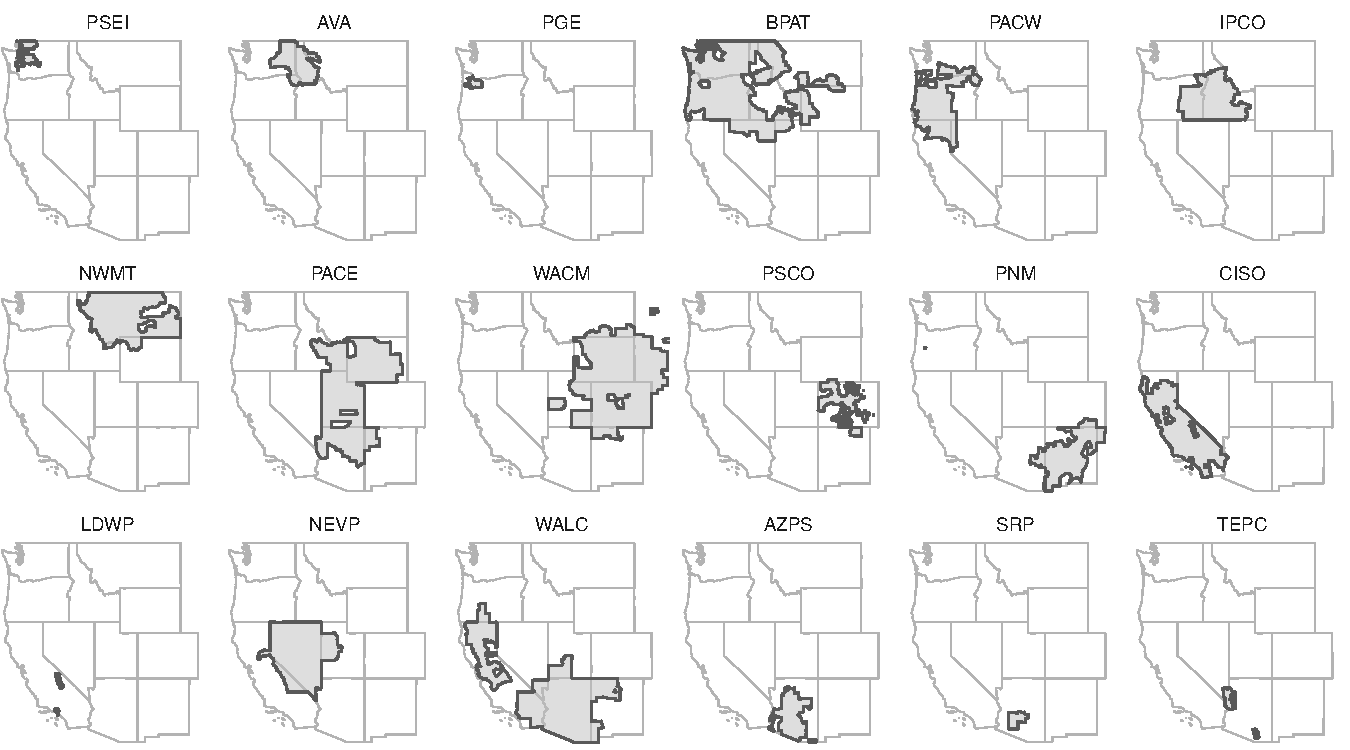
\includegraphics[width=\textwidth]{2-map_ba_panels}
    \caption{Balancing Authority (BA) control areas used in this study. These regions represent approximate geographic extent of each BA, not strict geographic boundaries. Newly sited wind and solar plants in this study are assigned to BAs based on the BA associated with the closest existing wind or solar plant.}
    \label{fig:map}
\end{figure}

Table \ref{tab:bas} shows the 18 BAs in this study along with the solar and wind capacity in gigawatts (GW). The table shows the capacity for the high renewable scenario in two key future years, 2035 and 2050 for the high renewable scenario. An analogous table for the business-as-usual scenario is presented in the supplemental material. Note that these potential infrastructure growth scenarios do not necessarily reflect long term utility planning. 

\begin{table} 
\begin{tabular}{llllllll}
     &                                        & solar & solar & solar & wind & wind & wind \\
BA   & BA Name                                & 2020  & 2035  & 2050  & 2020 & 2035 & 2050 \\\hline
AVA  & Avista                                 &   0.0 & 0.1 & 0.3 & 0.2 & 1.8 & 1.9  \\
AZPS & Arizona Public Service Company         &   0.8 & 7.2 & 10.6 & 0.2 & 5.2 & 8.2  \\
BPAT & Bonneville Power Administration        &   0.1 & 2.6 & 4.0 & 3.4 & 9.4 & 10.0  \\
CISO & Calif. Ind. System Operator            &   14.8 & 47.6 & 61.5 & 5.8 & 36.6 & 52.4  \\
IPCO & Idaho Power Company                    &   0.3 & 5.3 & 13.8 & 0.7 & 4.5 & 9.4  \\
LDWP & L.A. Dept. of Water and Power          &   1.0 & 3.1 & 2.3 & 0.4 & 4.7 & 5.6  \\
NEVP & Nevada Power Company                   &   1.6 & 18.7 & 23.9 & 0.1 & 1.4 & 2.1  \\
NWMT & NorthWestern Energy                    &   0.0 & 10.3 & 13.8 & 0.5 & 22.3 & 33.9  \\
PACE & PacifiCorp East                        &   1.3 & 59.1 & 65.8 & 2.7 & 23.1 & 31.2  \\
PACW & PacifiCorp West                        &   0.3 & 2.5 & 5.8 & 0.7 & 1.7 & 1.4  \\
PGE  & Portland General Electric              &   0.1 & 0.6 & 0.9 & 0.7 & 1.2 & 1.0  \\
PNM  & Public Service Company of N.M.         &   0.4 & 10.2 & 16.8 & 1.1 & 6.1 & 10.9  \\
PSCO & Public Service Company of Colo.        &   0.5 & 22.6 & 30.2 & 4.5 & 14.9 & 22.1  \\
PSEI & Puget Sound Energy                     &   0.0 & 0.1 & 0.2 & 0.5 & 2.9 & 3.4  \\
SRP  & Salt River Project                     &   0.3 & 4.3 & 4.1 & 0.1 & 0.1 & 0.4  \\
TEPC & Tuscon Electric Power Company          &   0.3 & 4.4 & 9.7 & 0.0 & 0.4 & 0.7  \\
WACM & WAPA* - Colorado-Missouri               &  0.2 & 8.4 & 20.1 & 0.8 & 7.9 & 14.4   \\
WALC & WAPA* - Lower Colorado                  &  0.1 & 4.4 & 6.9 & 0.3 & 4.5 & 4.7  \\
\hline
\end{tabular}
\caption{Balancing authorities used in the high renewable scenario in this study, with sited wind and solar capacity in gigawatts. *Western Area Power Administration}
\label{tab:bas}
\end{table}

We specifically focus on the daily time scale which can capture single- to multi-day duration compound droughts. Research using stochastic wind and solar forecast error and general intermittency already informs long-term planning and the need for intra-day storage and reserve requirements \cite{Ghosal2023}. However, there is currently no energy market in the U.S. that compensates for multi-day and week storage, which is typically addressed through bilateral agreements \cite{Bhatnagar2022}. Therefore, daily droughts are a relevant timescale to study. 

To identify droughts, hourly BA generation data is aggregated to daily based on the local time zone. Compound droughts are identified as consecutive days in which the total generation for both wind and solar falls below a fixed 10th percentile threshold for both wind and solar simultaneously -- the threshold is redefined for each infrastructure year to account for infrastructure buildout. Note that this threshold is arbitrary and in practice should be defined for each BA and generating resource based on regionally specific impacts. This definition of compound VRE drought is commonly used in the literature, though the threshold used varies between studies \cite{Allen2023a,Kittel2024}. A fixed threshold for the entire year is useful for determining the largest overall energy droughts, as opposed to a dynamic threshold which highlights seasonally abnormal droughts \cite{Bracken2024}. Looking at compound energy droughts is necessary both to represent the most extreme compound drought conditions and to capture the regional complementarity between wind and solar in the Western U.S.     

Drought duration is measured as the number of consecutive days meeting the drought criteria. Drought severity is measured as the cumulative energy deficit for both wind and solar below the drought threshold during a drought event, which can be expressed in megawatt-hours (MWh). Note that the threshold is dependent on the infrastructure year. To compare results across BAs, the severity is normalized by dividing by the maximum value in each BA, respectively. While this definition is a proxy for the true energy deficit which requires data on the full energy mix at every BA, it is a commonly used metric \cite{Allen2023a}.

\subsection{Multi-BA Droughts}

Droughts which occur simultaneously across multiple BAs have implications for the availability of energy on the market for inter-BA transfers as well as potential transmission needs. To identify multi-BA events we search both historical and future weather years for compound drought events which occur on the same day in one or more BA. Ideally, a connected event is a representation of a widespread weather pattern affecting multiple BAs. However, the Western U.S. is large enough that drought events in two BAs might not be caused by the same weather pattern. To visually filter out such events, BAs with a low number of connected events are deemphasized (i.e., shown with a lighter color) in the results. 

\section{Results}

This section presents the results for the high renewable scenario, the business as usual scenario results are presented in supporting information. 

\subsection{Compound VRE Drought Severity}

Our definition of compound VRE drought severity is the total energy deficit below the 10th percentile drought threshold. This threshold is redefined for each infrastructure year, thus as wind and solar capacity increases in the future, potential drought severity is expected to increase simply due to increasing capacity. The exact magnitude of severity increase is a complex function of the capacity increase, infrastructure placement, and future weather conditions. Figure \ref{fig:severity-future} shows the expected trend in severity in the high renewable scenario. The severity values are normalized by the maximum observed severity in each BA (represented by 1 on the y-axis) and which allows all severity to be measured between 0 and 1. Outliers have been removed for visual clarity. Note that the distribution in each infrastructure year reflects 40 years of future weather variability that we push through the on-the-ground infrastructure projected in a future year. The increase in drought severity reflects the dramatic growth in the wind and solar capacity necessary to meet high renewable climate goals. Every BA in this study is shown to experience several times more drought severity relative to 2020. This trend is robust across scenarios as well (see the supplemental material for business as usual scenario results). In a few BAs the severity dips in 2045. This is due to GCAM-USA simulations retiring all the existing plants (as of 2020) in that year and replacing them with new wind and solar facilities, sometimes falling in different BAs, temporarily decreasing the energy drought severity in some BAs. 

%\begin{itemize}
%    \item Are we building lots of renewables in BAs that show high proportion of severity 
%    \item Separate out susceptibility to energy drought based on building new renewables vs natural occurrence of drought 
%    \item Statistical test for increasing mean 
%\end{itemize}



\begin{figure}
\noindent
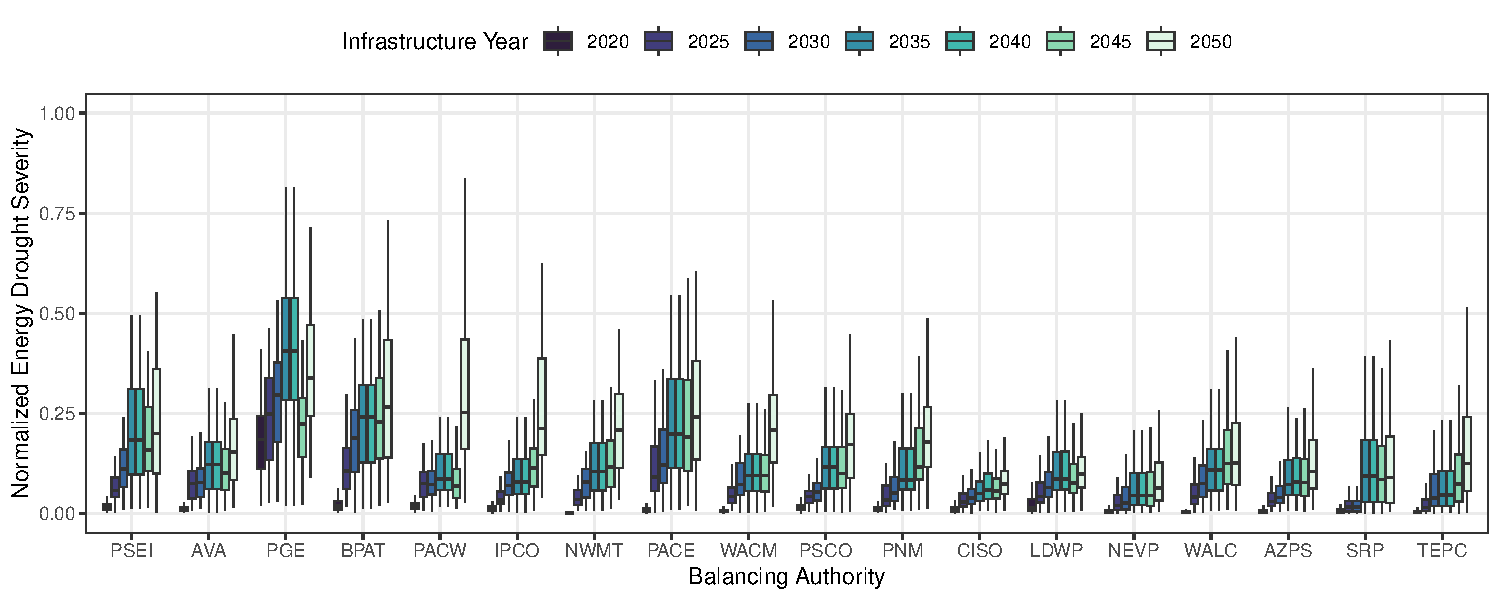
\includegraphics[width=\textwidth]{3-severity_future_nz_ws_droughts}
\caption{Energy drought severity (energy deficit below the 10th percentile) for the high renewable scenario which involves a high renewable grid by 2050. Climate variability is simulated for each infrastructure year using 40-years of rcp85hotter climate forcing. Severity has been normalized by the maximum value in each BA to allow the data to be compared across BAs and outliers have been removed for visual clarity.}
\label{fig:severity-future}
\end{figure}

\subsection{Future Climate Impact on Compound VRE Drought Severity}

The increase in energy drought severity seen in the previous section is a combination of infrastructure and climate signals. To test the influence of future climate alone on compound VRE drought severity, energy droughts under future infrastructure were also computed with historical (1980-2019) climate. The normalization of VRE drought is computed the same across both historical and with future climate. The difference is then computed between the normalized severity in each pair of years of the historical and future periods, which is enabled by TGW climate datasets where the historical sequencing is repeated in the future. Future climate (i.e., future - historical climate forcing) has a limited effect on the average drought severity (Figure \ref{fig:severity-diff}). All distributions encompass zero and few BAs show any systematic trend in the mean. In the high renewable scenario, 96.3\% of future infrastructure years tested as having a mean equal to zero (t-test at 1\% significant level) and 100\% of of future infrastructure years tested to have a mean the same as the baseline year (two-sided t-test at 1\% significance level), with the business-as-usual scenario testing at 96.3\% and 97.2\% respectively. 

Future climate provides little to no contribution to the increase in future severity but it does impact the variability, a statistically significant increase in variance (F test at 1\% significance level) exists in 97.2\% of future infrastructure years compared to the baseline 2020 infrastructure in the high renewable scenario and 94.4\% in the business as usual scenario. These results indicate that future climate may increase compound VRE drought variability which should inform storage and transmission designs and financial stability studies. 


\begin{figure}
\noindent
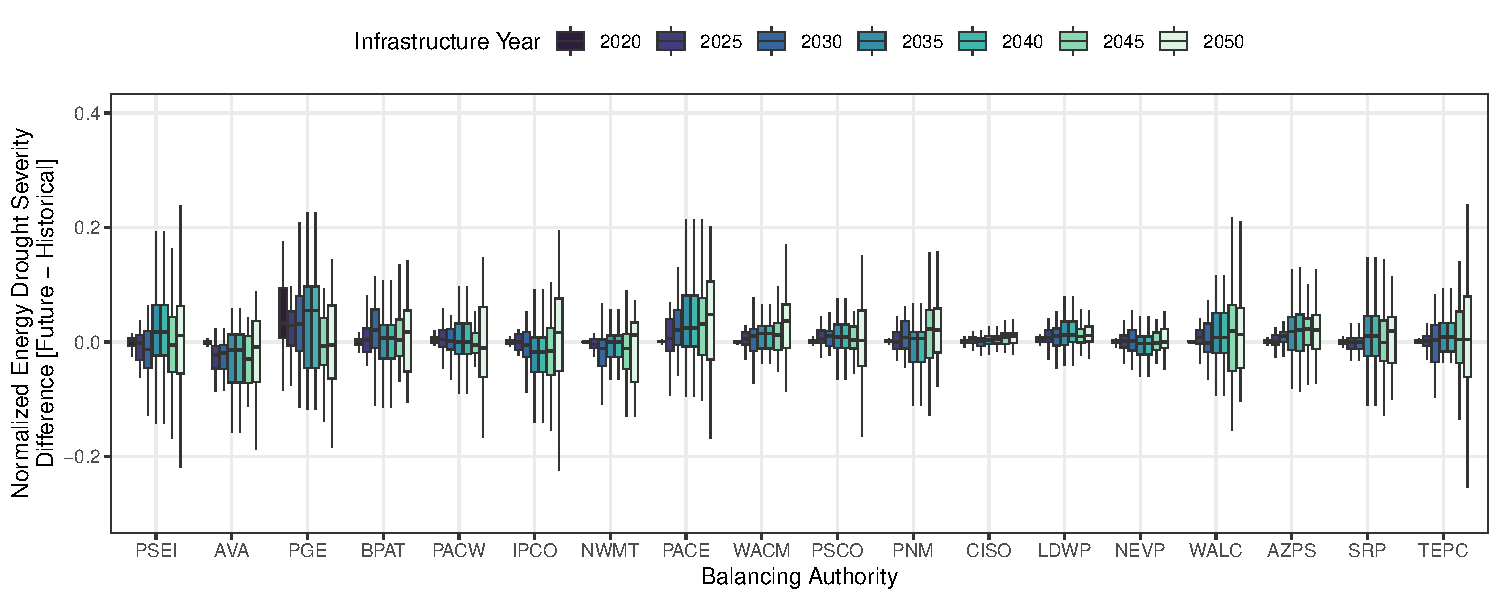
\includegraphics[width=\textwidth]{4-severity_diff_hist_future_nz_ws_droughts}
\caption{Difference in average annual normalized energy drought severity between the future and historical periods for the high renewable scenario, which involves a high renewable grid by 2050. Severity has been normalized per BA to allow the data to be compared across BAs.}
\label{fig:severity-diff}
\end{figure}

\subsection{Duration}

No significant trend in drought duration was detected across infrastructure or climate scenarios (Figure \ref{fig:duration}). Note average duration was 1 day in all cases becasue distribution of drought duration is heavily skewed. BAs in California -- California Independent System Operator (CISO) and Los Angeles Department of Water and Power (LDWP) -- exhibit some of the longest duration compound droughts, which is consistent with the historical analysis in \citeA{Bracken2024}.

This null result likely stems from the design of the TGW climate forcing. The TGW data relies on a perturbation approach in which 40-years of historical events (1980-2019) are replayed in the future with additional warming levels applied to the boundaries of the downscaling model to reflect the future climate signal. The sequencing, including the duration, of historical events is maintained in the future. The atmospheric dynamics that resulted in, for example, a 3-day historical heat wave will be maintained in the future even though the intensity of the heat wave will obviously be hotter. For this reason any results related to changes in the duration of extreme events using the TGW forcing should be interpreted with caution.  

\begin{figure}
\noindent
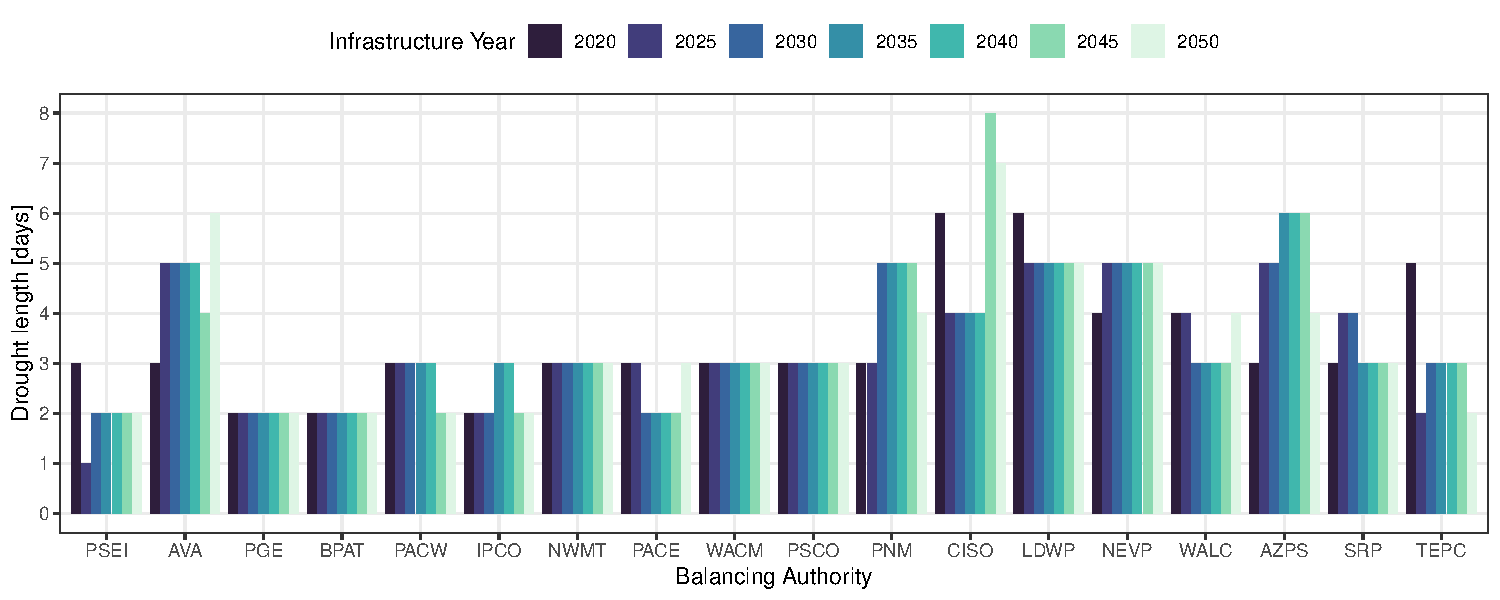
\includegraphics[width=\textwidth]{5-duration_future_nz_ws_droughts}
\caption{Maximum compound VRE drought duration for the high renewable scenario, which involves a high renewable grid by 2050. Note that the figure does show boxplots, but in most BAs the distribution of drought duration is heavily skewed such that most boxes are collapsed on at the lowest value. }
\label{fig:duration}
\end{figure}

\begin{figure*}
\noindent
\centering
\begin{adjustwidth}{-35mm}{-35mm}
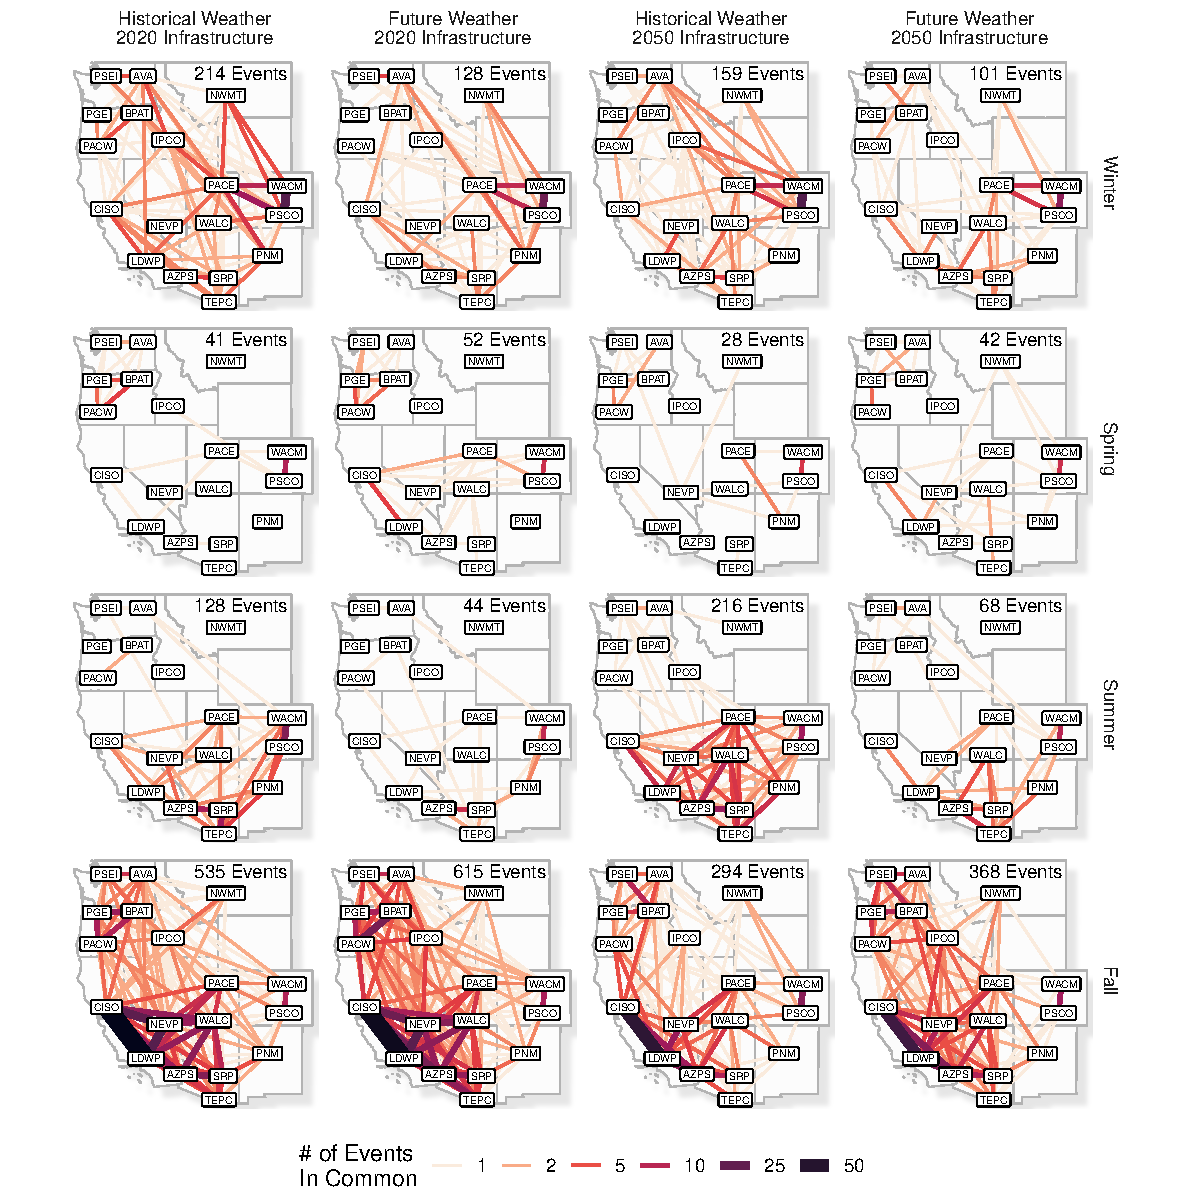
\includegraphics[width=\linewidth]{6-spatial_connectivity_seasonal_nz_ws_droughts}
\end{adjustwidth}
\caption{Seasonal compound energy drought co-occurrence between BAs for the high renewable scenario using historical weather with 2020 infrastructure (first column) and future weather with 2020 infrastructure (second column), historical weather with 2050 infrastructure (third column), and future weather with 2050 infrastructure (fourth column). The rows indicate the seasons. A line is drawn between two BAs if at least one energy drought occurred on the same day. The thickness and color of the line represent the number of events in common between a pair of BAs.}
\label{fig:connectivity}
\end{figure*}

\subsection{Spatial Co-occurrence}

Figure \ref{fig:connectivity} shows the seasonal co-occurrence of compound VRE droughts between BAs for the high renewable scenario. Each row represents a season (winter [DJF], spring [MAM], summer [JJA], fall [SON], from top to bottom), the left column represents historical weather years with 2020 infrastructure, the baseline scenario. The middle left column represents future weather years with 2020 infrastructure which indicates the influence of future climate. The middle right column shows historical weather with 2050 infrastructure, which indicates the influence of infrastructure growth. The right column represents future weather years with 2050 infrastructure which combines the effects of future climate and infrastructure. In the top right of each panel is the number of events in the 40 year period represented in that panel, which demonstrates the seasonality of compound VRE droughts. Winter shows widespread co-occurrence, which is the strongest in the eastern part of the interconnection, and overall less co-occurrence in the future period. Spring has the weakest co-occurrence as well as the lowest occurrence of events, suggesting that weather patterns that cause droughts are less frequent and more localized in this season. In summer, co-occurrence is concentrated in the southwest, indicating potential for issues in a region increasingly dependent on solar energy \cite{Tabassum_2021}. In fall we observe the most co-occurrence with the strongest connectivity occurring along the coast. Fall is typically the lowest season for hydropower in this region which indicates potential for compound hydropower droughts. In most seasons, the connection between CISO and LDWP (in California) and WACM and PCSO in (Colorado) are strong, likely due to sharing overlapping territory and similar weather patterns (Figure \ref{fig:map}).

To quantify the change in connectivity between the historical and future periods, we computed the difference between the number of connected events under future and historical conditions holding either infrastructure or climate constant. Figure \ref{fig:connectivity-trend} shows this difference broken out by season and the number of BAs included in a connected event. The left panel shows the climate influence which is the difference between the number of events in the future and historical periods using 2050 infrastructure (columns 3 and 4 in Figure \ref{fig:connectivity}). The right panel shows the infrastructure influence between 2050 and 2020 infrastructure using future weather conditions (columns 4 and 2 in Figure \ref{fig:connectivity}). Negative values indicate fewer events under future conditions. 

Under the influence of future climate, summer and winter exhibit significantly fewer co-occurring events. Conversely in fall and spring, future climate causes an increase in the number of co-occurring events, with a notable increase of more widespread events in the fall, indicating a shift toward more widespread weather patterns that contribute to compound VRE drought in this season. Infrastructure growth has the effect of decreasing the number of co-occurring events in winter, spring, and fall and slightly increasing the number co-occurring events in the summer. While counterintuitive, this effect is likely due to the increase in the density of wind and solar plants such that that more plants in a particular BA must be in drought conditions simultaneously for the whole BA to experience drought. Interestingly, in the fall, future climate and infrastructure growth induce the opposite effect on the number of co-occurring events, with the infrastructure effect winning out and causing an overall decrease when the effects are combined. 

\begin{figure}
\noindent
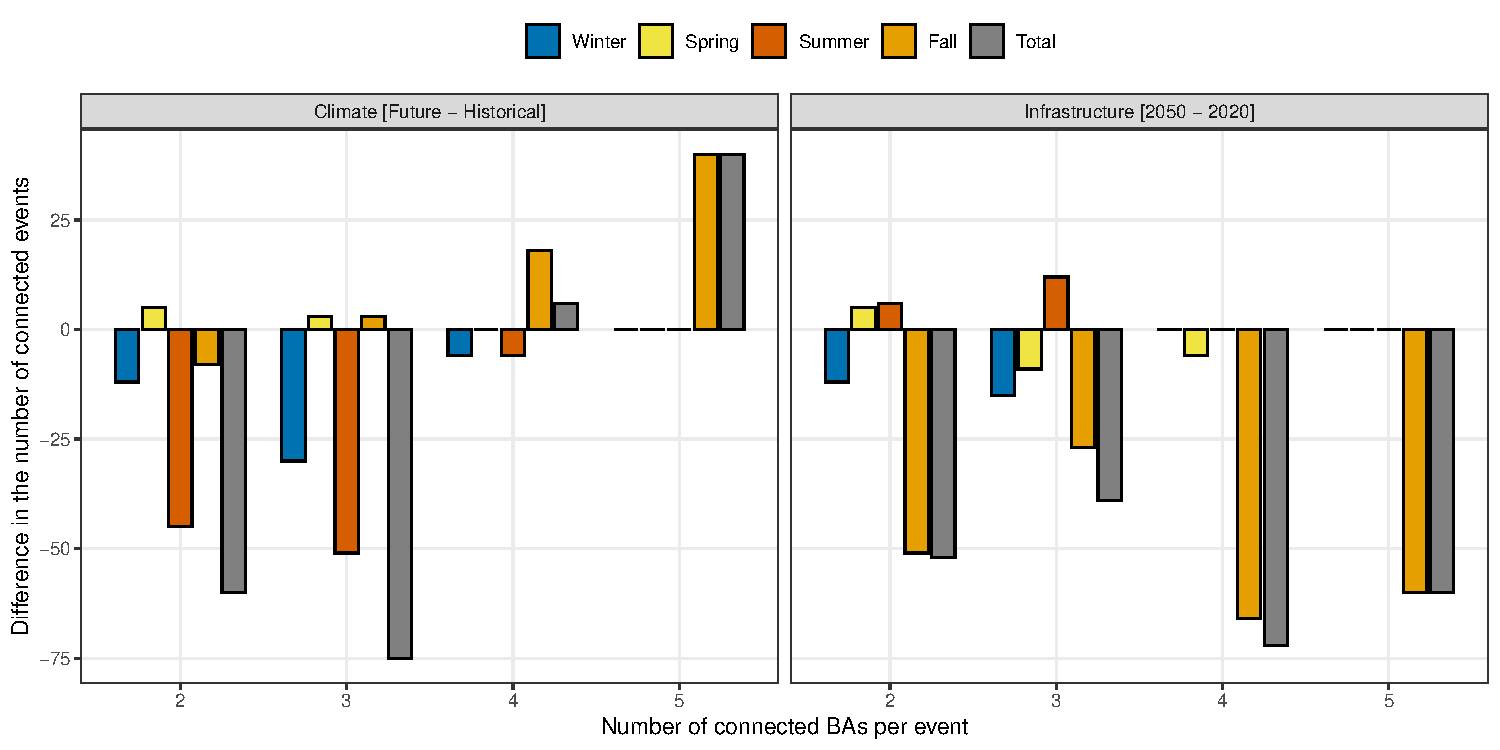
\includegraphics[width=\textwidth]{7-connected_event_diff_nz_ws_droughts}
\caption{The difference between the number of multi-BA compound energy droughts in each season for the high renewable scenario. The left panel shows the climate influence by differencing the future weather and historical weather periods using 2050 infrastructure. The right panel shows the infrastructure influence by differencing the 2050 and 2020 infrastructure scenarios both using future weather. Negative values indicate fewer connected events in the future period.}
\label{fig:connectivity-trend}
\end{figure}

\section{Discussion}

The results in this study are limited to two infrastructure scenarios and one climate-socioeconomic scenario (SSP2-RCP8.5hotter). This is primarily due to resource constraints as running the entire chain of necessary models to build the infrastructure is very time and resources intensive. Ideally we would also have examined a more moderate climate scenario. Because we used a very hot climate scenario (rcp85hotter) this study represents an upper end of the feasible future scenarios, in which the climate stress on the grid is high. Our results show that future trends in severity, duration, and connectivity are robust across both infrastructure scenarios, albeit with lower severity in the business as usual scenario due to lower growth in renewable capacity. 

Changes to compound VRE droughts in the future will be due to a combination of changing climate and infrastructure buildout. As renewable capacity increases in both the high renewable and business-as-usual scenarios, we see a dramatic increase in the energy drought severity. Recall that compound VRE drought severity is defined as the deficit below the 10th percentile threshold, updated for every infrastructure year. Based on this definition, this increase in severity is expected but the degree of increase is quite dramatic, ranging from 5 to over 200 times the severity of the historical infrastructure in some BAs. The severity is directly relatable to the quantity of energy that, given energy demands, must be met with other sources of generation and storage. The sizing and operational management of local energy storage, and regional transmission needs assessment are one of the primary applications of this work.  

The experimental design of this study allows us to isolate future climate and infrastructure effects on compound VRE drought severity. We were able to isolate the effects of future climate by differencing the historical and future weather periods and while holding the infrastructure constant. Future climate was shown to have a limited effect on compound VRE drought severity, but causes the variability of droughts to increase in the future. Variability in this case refers to the variance of the severity of compound VRE droughts which indicates a need for increasingly robust storage and transmission solutions to mitigate. 

Compound VRE drought duration was found to have no significant trend under future infrastructure or climate conditions. We expected the contribution due to future climate alone to be limited due to the construction of the meteorology data used (see the next section for further discussion on this limitation). Infrastructure having a limited effect on compound VRE drought duration implies that building more wind and solar will neither shorten nor lengthen those VREs and they need to be specifically mitigated by other technologies in the resources adequacy process. We therefore recommend that energy drought scenarios be added to seasonally critical event periods represented in capacity expansion models with explicit representations for storage and transmission expansions. We acknowledge the large uncertainties in projected future infrastructure scenarios \cite{Browning_2023}. We also note that to mitigate this currently unrepresented `climate threat', capacity expansion models need to achieve a spatial resolution of BA, or State scale at maximum, and explicit representation of representative periods that consider coincidence in wind, solar and load in time and across regions. 

The final set of results from this study are related to the spatial extent of VRE droughts and how that might change in the future due to either changing climate or infrastructure growth. To do this, we mapped the spatial connectivity of VRE drought events to determine how often droughts occurred simultaneously in two or more BAs. We found that the pattern of spatial co-occurrence is highly seasonally dependent due to the seasonal seasonal cycle of drought frequency, with the most co-occurring events in the Winter and Fall. One surprising result is that the number of compound drought events decreases in most seasons due to both changing climate and infrastructure scenarios, contributing to fewer connected events. Fewer events under future climate may indicate that some seasons will have less widespread weather patterns which contribute to compound VRE drought. The notable exception is that future climate increases the number of the largest co-occurring events in the fall (i.e., those affecting 4 and 5 BAs simultaneously), which indicates a shift in that seasons toward drought-inducing weather patterns that affect more regions simultaneously. Fall is typically when hydropower production in the western U.S. is lowest. Infrastructure growth caused fewer drought events in every season except summer. This is likely a consequence of the density of the wind and solar generation in our future scenario, which creates more strict conditions for compound droughts over large BA areas. The combined effect of future climate and infrastructure led to equal or fewer co-occurring droughts in every season which is a benefit of large scale deployment of variable renewable generation and a net positive result for a future high renewable grid.


\section{Limitations}

Due to the nature of the TGW meteorology data used in this study, we were able to robustly isolate the impact of climate from infrastructure buildouts on energy drought intensity and variability. However we were not able to comprehensively assess the frequency of future drought events. Because the future projections in the TGW dataset are based on the historical timing and sequencing of events like heat waves and cold snaps, the future frequency of those events will not change despite the warming signal. This is an unfortunate limitation as the frequency of energy droughts is a concern for future grid reliability. This could be overcome by incorporating model projections from datasets such as the Coupled Model Intercomparison Project (CMIP). Though, as \citeA{Kapica_2024} show, the variability between climate models can be large so care needs to be taken when selecting individual models. That aspect of future energy droughts is left for future studies.

No hydropower was considered in this study. In the Western U.S., hydropower is an important resource for mitigating energy drought due to its storage capacity and thus flexibility to adjust the timing of generation. The time scale of hydrologic drought (months to years) is much longer than energy droughts (hours to days) and is typically omitted from VRE drought studies. The interaction between these two types of drought needs further study, particularly on the seasonal scale where hydropower affects seasonal power grid operations across the whole western interconnect \cite{Voisin_2018,Hill_2021} and might help in evaluating the value of long term duration storage such as hydrogen.

In this study, we do not quantify the impact of compound VRE droughts on grid operations and specifically the potential threat to power grid reliability. Capacity expansion models are often limited to generator capacity expansion while emerging models now also include transmission expansion and new transmission paths \cite{Gonzalez_Romero_2020}. This research provides unique datasets and characterization of extreme low renewable generation events that can inform those emerging models and address the tradeoffs between storage and transmission. At a more regional scale, the provided datasets can also inform hybrid systems with batteries, hydropower, and especially valuation project for pumped storage hydro \cite{Francois2016}. 
%Such a model would include real time energy demands, outages and ramping constraints.  

\section{Conclusions}

In this study we have presented the first analysis of its kind to examine future compound variable renewable energy (VRE) droughts under a changing climate and evolving infrastructure in the Western US. VRE droughts are a natural part of any energy systems wind and solar technology portfolio and will plant an even larger role in a high renewable energy system where droughts must be mitigated through energy storage or interregional energy transfers. We examine compound wind and solar energy droughts under a RCP 8.5 warming scenario with both high renewable and business-as-usual scenarios out to 2050. Realistic future buildouts of wind and solar are achieved with an interconnected chain of models involving capacity expansion, plant siting, energy prices, and renewable electricity generation modeling. 

The severity of compound droughts, as measured as the shortfall below the 10th percentile of daily total generation, is expected to increase in the future, primarily due to the dramatic buildout of wind and solar generation in our scenario. In some BAs, energy drought severity increases by as much as 200\% over historical conditions. We demonstrate that future climate does not impact the mean severity of energy droughts, but will cause the variability of the severity of compound drought events to increase in the future. This finding has implications for sizing and managing energy storage and regional transmission capacity necessary to mitigate energy droughts. No trend in compound drought duration was detected due to furture infrastructure buildout or climate. 

Co-occurrence of compound VRE drought across BA regions was also considered, which can further inform the trade off between regional storage and transmission needs. Co-occurrence in the Western U.S. interconnect has strong seasonal patterns and is affected by both future climate and infrastructure growth in the future scenarios. Winter and fall show the most widespread and strongest drought co-occurrence while the spring is the weakest. Summer co-occurrence is primarily isolated to the Southwest. The combined effect of climate and infrastructure growth is equal or fewer co-occurring events in every season, a positive result for a future high renewable grid. The most notable effect of future climate was in the fall where we observed a shift toward co-occurring events which effect larger number of regions simultaneously. This finding also has implication on modeling needs in capacity expansion models to address the VRE threats. Futhermore, the fall is when hydropower is typically the lowest in the Western U.S., indicating the possibility of compound wind-solar-hydro droughts, a topic which needs further study. These findings need to be evaluated as part of future work with seasonal hydropower capabilities and potential shifts in seasonal load peaking across the region. 

 
%%


%%%%%%%%%%%%%%%%%%%%%%%%%%%%%%%%%%%%%%%%%%%%%%%
%
% DATA SECTION and ACKNOWLEDGMENTS
%
%%%%%%%%%%%%%%%%%%%%%%%%%%%%%%%%%%%%%%%%%%%%%%%

\section*{Open Research Section}
Data for historical generation for existing EIA plants is found in \citeA{Bracken2023a}. Data for historical and future generation data based on CERF cited plants is found is \citeA{Bracken2024a}. Code to conduct the analysis can be found in \citeA{bracken2025-future-drought-code}.

\acknowledgments
This research was supported by the Laboratory Directed Research and Development (LDRD) Program at Pacific Northwest National Laboratory (PNNL). The study leverages the TGW climate datasets developed by U.S. DOE Office of Science multisector dynamics program as part of the IM3 and HyperFACETS projects. The CERF siting model was developed under the IM3 project and was enhanced as part of the GODEEEP project. The GCAM-USA model is also developed and supported by the U.S. DOE Office of Science mutisector dynamics program under the IM3 and GCIMS projects and was enhanced as part of the GODEEEP project to represent high renewable economies.

This material was prepared as an account of work sponsored by an agency of the United States Government.  Neither the United States Government nor the United States Department of Energy, nor the Contractor, nor any or their employees, nor any jurisdiction or organization that has cooperated in the development of these materials, makes any warranty, express or implied, or assumes any legal liability or responsibility for the accuracy, completeness, or usefulness or any information, apparatus, product, software, or process disclosed, or represents that its use would not infringe privately owned rights.

Reference herein to any specific commercial product, process, or service by trade name, trademark, manufacturer, or otherwise does not necessarily constitute or imply its endorsement, recommendation, or favoring by the United States Government or any agency thereof, or Battelle Memorial Institute. The views and opinions of authors expressed herein do not necessarily state or reflect those of the United States Government or any agency thereof.  Pacific Northwest National Laboratory is operated by Battelle for the U.S. Department of Energy under Contract DE-AC05-76RL01830. 


%%%%%%%%%%%%%%%%%%%%%%%%%%%%%%%%%%%%%%%%%%%%%%%
% REFERENCES and BIBLIOGRAPHY
%
% \bibliography{<name of your .bib file>} don't specify the file extension
% don't specify bibliographystyle
%
%%%%%%%%%%%%%%%%%%%%%%%%%%%%%%%%%%%%%%%%%%%%%%%

\bibliography{refs}


%Reference citation instructions and examples:
%
% Please use ONLY \cite and \citeA for reference citations.
% \cite for parenthetical references
% ...as shown in recent studies (Simpson et al., 2019)
% \citeA for in-text citations
% ...Simpson et al. (2019) have shown...
%
%
%...as shown by \citeA{jskilby}.
%...as shown by \citeA{lewin76}, \citeA{carson86}, \citeA{bartoldy02}, and \citeA{rinaldi03}.
%...has been shown \cite{jskilbye}.
%...has been shown \cite{lewin76,carson86,bartoldy02,rinaldi03}.
%... \cite <i.e.>[]{lewin76,carson86,bartoldy02,rinaldi03}.
%...has been shown by \cite <e.g.,>[and others]{lewin76}.
%
% apacite uses < > for prenotes and [ ] for postnotes
% DO NOT use other cite commands (e.g., \citet, \citep, \citeyear, \nocite, \citealp, etc.).


\end{document}




